\documentclass{article}
\usepackage{xcolor}
\usepackage{graphicx}
\usepackage{caption}
\usepackage{subcaption}
\usepackage[utf8]{inputenc}
\usepackage[T1]{fontenc}
\usepackage[francais]{babel}
\usepackage{hyperref}
\hypersetup{
colorlinks=true,
breaklinks=true,
urlcolor= blue,
linkcolor= black,
citecolor=black,
}
\usepackage{enumitem}
\usepackage{float}
\usepackage{pifont}

\addtolength{\textwidth}{3cm}
\addtolength{\oddsidemargin}{-1.5cm}


\begin{document}
%-----------------------------------------------------------------------
\hrule
\begin{center}
\Huge {\textsc{CULTUR'ADVISOR - Développement d'une plateforme}}
\end{center}
\hrule
\vspace{10mm}
\begin{center}
\Large \textsc{Master 2 IMIS \\ Année 2022-2023}
\end{center}
\vspace{15mm}
\begin{figure}[H]
\hspace{-10mm}

\includegraphics[scale = 0.5]{images/logo_advisor.png}
\end{figure}
\vspace{20mm}

\begin{center}
\vfill{\Large \textsc{ Présenté par : Barodine Anaël, Mbelek-Nouga Paul-Dubien, TESSIER Adrien, Ververke Xavier \\ Encadré par : Tandjaoui Rosa et Hakim Aoudia}}
\end{center}
\begin{figure}[H]
\hspace{-0mm}

\includegraphics[scale = 0.4]{images/logo_orleans.png}
\hspace{10mm}

\includegraphics[scale = 0.4]{images/logo1.png}
\hspace{10mm}
\includegraphics[scale = 0.15]{images/logo_dill.png}
\end{figure}
\newpage
%-----------------------------------------------------------------------
\vspace*{\stretch{1}}
\begin{center}
\Large\bfseries
\title -Remerciements
\end{center}
\hspace{4.5mm} 
Tout d’abord, nous tenons à remercier Rosa Tandjaoui, notre mentor, et Matthieu Exbrayat notre encadrant universitaire de nous avoir accompagnés et guidés pour ce projet.

Nous voulons aussi remercier toutes les personnes qui ont contribué au succès de ce projet et qui nous ont aidés lors de la rédaction de ce rapport.


\vspace*{\stretch{1}}
\newpage
%-----------------------------------------------------------------------
\tableofcontents
\newpage %aller a la page suivante
%-----------------------------------------------------------------------
\section{contexte du projet}
À la croisée de l’agenda culturel, du média, du magazine et du réseau social, Cultur’Advisor est un espace de productions, de consultations et d’échanges autour de la culture.\\
En France, il n’existe pas de base de données regroupant l’ensemble des produits culturels du territoire. Il existe bien de telles bases mais elles sont restreintes à de plus petites zones géographiques (département, région) ou à certains événements précis (festivals...). Tout cela rend plus difficile pour le public de les découvrir.\\
L’objectif de l’entreprise est donc de faciliter l’accès à la culture en aidant les acteurs à trouver de nouveaux publics, améliorer leur visibilité, augmenter leur fréquentation et pour le public, à trouver l’expérience culturelle qui leur ressemble, leur correspond car encore aujourd’hui, beaucoup de produits ou services culturels ne trouvent pas leurs clientèle et les clients finaux ne sont souvent pas informés de l’offre, ni même conscient de son intérêt.\\
Pour cela le projet consiste en la réalisation d’une application afin de permettre aux utilisateurs de découvrir plus facilement cette culture en France.
\newpage

\section{organisation de l'équipe}

\subsection{Moyens de communication}
Après avoir été attribué à ce projet, nous avons rencontré notre mentor aux dill Bootcamp à Bourge et nous avons fait une première réunion en sa compagnie afin de découvrir plus en détails ce que nous devrions faire pour ce projet. \\
À la suite de cette réunion, nous avons créé un dépôt git sur GitHub afin que nous puissions bien travailler ensemble sur ce projet. Ensuite, pour pouvoir discuter entre étudiants de ce groupe et connaître l’avancement de chacun, nous avons utilisé Discord pour pouvoir partager nos ressources et nos rendus.\\
Afin que notre mentor puisse connaître l’avancement de notre projet, nous avons utilisé Whatsapp et fait plusieurs réunions avec elle.


\subsection{Répartitions des tâches}
Afin de mener ce projet à bien, nous avons commencé par se répartir les différentes tâches du projet.\\
Nous avons, avec notre mentor défini ces différentes tâches qui sont de récupérer l’ensemble des données disponible sur les API, les rassembler et les uniformiser, en faire une base de données, puis pouvoir faire des requêtes sur ces données en fonction des utilisateurs.\\
Pour commencer, Anaël s’est occupé de créer le serveur Flask ainsi que de regarder comment récupérer les données sur les API.\\
Ensuite, Adrien s’est occupé de récupérer le reste des données ainsi que de normaliser ces données.\\
Et enfin, Xavier s’est occupé de créer une base de données à partir des données normalisées.\\
Pour finir, il nous restera à faire des requêtes sur cette base de données.
\newpage

\section{Projet}

\subsection{Mis en place du projet}
Premièrement, nous avons d’abord commencé par choisir ensemble un langage dans lequel nous pourrions réaliser ce projet et nous avons choisi Python qui nous permettait de créer un serveur Flask et de bien manipuler les différentes données que nous avons. Flask permet de mettre en place un serveur web. Il est chargé de recevoir des requêtes HTTP et éventuellement d’y répondre. Il suffit de déterminer les URL, appelés routes, qui réceptionnent les requêtes et les traitent.
\begin{figure}[H]
\hspace{-0mm}

\includegraphics[scale = 0.55]{images/python.png}
\hspace{10mm}

\includegraphics[scale = 0.5]{images/flask_logo.png}
\end{figure}

\subsection{Création du serveur Flask}
La création d’un serveur Flask est simple. Pour cela, il faut importer la bibliothèque Flask et appeler le constructeur du même nom. Ensuite il faut rédiger les routes et le traitement des requêtes. Cela se fait en écrivant une méthode qui sera le traitement de la requête à laquelle on ajoute une annotation @app.route qui prend en paramètre la route d’où doit venir la requête.
\begin{figure}[H]
\center
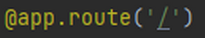
\includegraphics[scale = 0.7]{images/flask.png}
\caption{Annotation définissant une route}
\end{figure}


\subsection{Récupération des données}
Une fois le serveur Flask mis en place, il faut maintenant pouvoir récupérer les différentes données disponibles. Pour cela, nous avons eu par notre mentor une liste d’API contenant différents produits culturels à récupérer et nous a\\vons commencé par analyser ces différentes bases de données.
Ensuite, nous avons récupéré chaque colonnes de ces bases de données puis nous en avons fait un tableau comme nous montre les 2 images ci-dessous qui correspondent à 2 bases de données que nous avons récupérés.
\begin{figure}[H]
\hspace{-25mm}
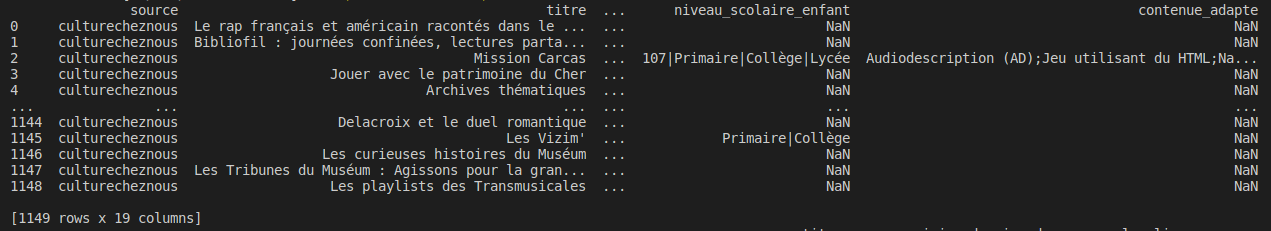
\includegraphics[scale = 0.44]{images/culturecheznous.png}
\caption{Dataframe contenant les données de culture chez nous}
\end{figure}
\begin{figure}[H]
\hspace{-25mm}
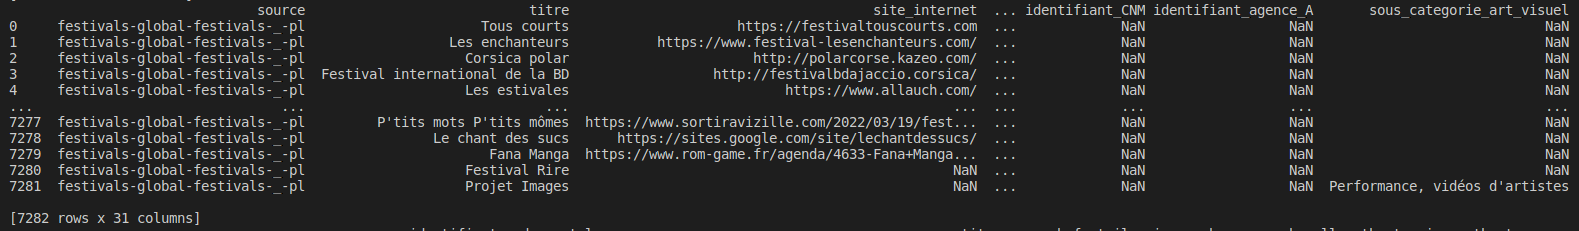
\includegraphics[scale = 0.354]{images/festivals.png}
\caption{Dataframe contenant les données des festivals en France}
\end{figure}
Nous avons donc récupéré chaque colonnes une à une de ces bases de données ce qui nous donne en sortie 5 tableaux avec respectivement 19, 22, 31, 35 et 17  colonnes.\\
Ensuite, avant de regrouper tous ces tableaux en un, nous avons déjà fait une normalisation à l’intérieur de ces tableaux car par exemple dans un tableau, nous avions 2 colonnes différentes qui représentaient le lien d’un site internet (lien1 et lien2) et nous l’avons regrouper en une seule colonne sous le nom de (site-internet) comme le montre l’image ci dessous.

\begin{figure}[H]
\center
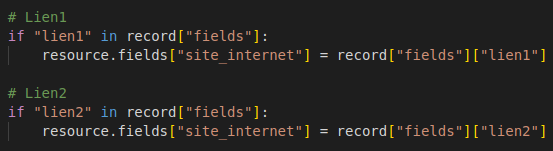
\includegraphics[scale = 0.6]{images/liens.png}
\caption{Exemple de deux colonnes d’un tableaux rassemblé en une}
\end{figure}

\subsection{Normalisation des données}
Après avoir récupéré ces données et les avoir mis dans des tableaux différents, nous devions donc les rassembler et les normaliser.\\
Pour cela, nous avons utilisé un Dataframe afin de mettre tous les tableaux récoltés dans un seul.\\
Pour tous les tableaux que l’on a, nous avons regardé les colonnes qui contenaient les mêmes données mais qui avaient des noms différents puis on a changé ces noms de colonnes afin que chaque tableau de données qui contenait les mêmes données ait le même nom de colonnes afin qu’il soit normalisé.\\
On a donc pu réduire le nombre de colonnes dans ce dernier Dataframe ci-dessous pour passer de 124 colonnes à 90.

\begin{figure}[H]
\hspace{-25mm}
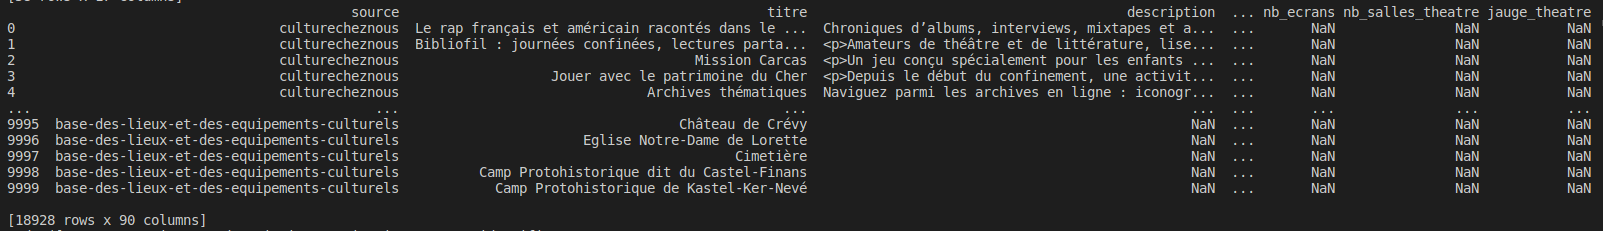
\includegraphics[scale = 0.35]{images/dataframe_final.png}
\caption{Dataframe contenant toutes les données après la normalisation}
\end{figure}
Une fois qu’on a construit ce Dataframe avec toutes les données normalisées, nous l’avons transformé en fichier CSV Pour pouvoir ensuite récupérer ce CSV et en faire une base de données.\\
Nous avons aussi remarqué qu’en normalisant tous ces tableaux en un seul Dataframe, Nous avons beaucoup de valeurs Null car par exemple sur le Dataframe ci dessus nous voyons que le tableau culturecheznous contient une description mais le tableau base-des-lieux-et-des-equipements-culturels n’en contient pas ce qui pourrait poser d'éventuelle problèmes lors des requêtes que nous ferons par la suite.

\subsection{Mise sous forme de base de données}
Une fois les données récupérées et stockées sous CSV, il a fallu le parcourir ligne par ligne pour remplir la base de données. Pour réaliser cela nous avons utilisé une base de données MySQL.\\
Malgré le fait que les données soient normalisées, un problème subsiste, les champs sont de longueur variable. Par exemple, le champ description est parfois absent dans certaines lignes mais une autre contient une portion entière de code HTML. Pour permettre l’insertion de ces variables à taille indéterminée nous les stockons sous le type Text.

\subsection{Requêtes}
Le stockage sous forme de base de données nous permettra de réaliser des requêtes sur les données. Nous pourrons donc obtenir des informations en fonction de paramètres.

\section{Conclusion}
Pour conclure, lors de ce projet, nous avons répondu au besoin initial qui était de rassembler toutes les données culturelles afin de les mettre en valeurs pour le public.\\
Malgré quelques soucis lors de la lecture des données disponible sur les différentes API et la mise en place de la base de données, nous avons pu surmonter ces erreurs en nous entraidant.\\
Nous avons pris un peu de retard au début de ce projet à cause d’une mauvaise compréhension du travail réalisé ainsi que l’absence d’un des membres de notre équipe mais nous avons quand même pu continuer à mener ce projet à bien et qui continuera d’être amélioré jusqu'à la fin.
\end{document}